\subsection{Ergebnisse und Auswertung} \label{sec:ErgebnisseFES}
  
  In Tabelle \ref{tab:ErgebnisseFES} befinden sich die Ergebnisse der Kalibrier- und Probemessungen. Die Kalibriergerade ist in Abbildung \ref{fig:KalibriergeradeEisen} dargestellt. Folgende Parameter der Kalibriergeraden wurden bestimmt: Steigung $b = \SI[mode=text,separate-uncertainty]{23.7(2)}{AU\per ppm}$, Ordinatenabschnitt $a = \SI[mode=text,separate-uncertainty]{32(3)}{AU}$, Bestimmtheitsmaß $R^2 = 0.9990$, Reststandardabweichung $s_y = 5.776$, F-Wert $F = 12584.75$ und Freiheitsgrade $df = 13$. Die Konzentration der Probe, $c_{Probe}$ wird durch Umstellen der Kalibriergeraden auf $x$ berechnet:
  
    \begin{equation}
      c_{Probe} = \frac{\overline{y_{Probe}} - a}{b} = \SI[mode=text]{10.5}{ppm}.
    \end{equation}
  Der Vertrauensbereich für $\alpha = 0.05$ ($N = 15, t = 2.16$) kann über die Standardabweichung der Kalibriergeraden berechnet werden:
  
    \begin{equation}
      \begin{split}
        s_c &= \frac{s_y}{b} \sqrt{\frac{1}{N} + \frac{1}{m} + \frac{\left(\overline{y_{Probe}} - \overline{y}\right)^2}{b^2 \sum_{i=1}^N \left(x_i - \overline{x}\right)^2}} \\
            &= \frac{5.776}{23.7} \sqrt{\frac{1}{15} + \frac{1}{6} + \frac{\left(280 - 268\right)^2}{23.7^2 \cdot 750}} = \SI[mode=text]{0.118}{ppm} \\
     \Rightarrow T_c &= t s_c = \SI[mode=text]{0.255}{ppm}.
      \end{split}
    \end{equation}
  Damit ist das Ergebnis: $c_{Probe} = \SI[mode=text, multi-part-units = brackets, separate-uncertainty]{10.5(3)}{ppm} \left(N = 15, s_c = \pm \SI[mode=text]{0.12}{ppm}, \alpha = 0.05\right)$.
  
  \begin{figure}[H]
    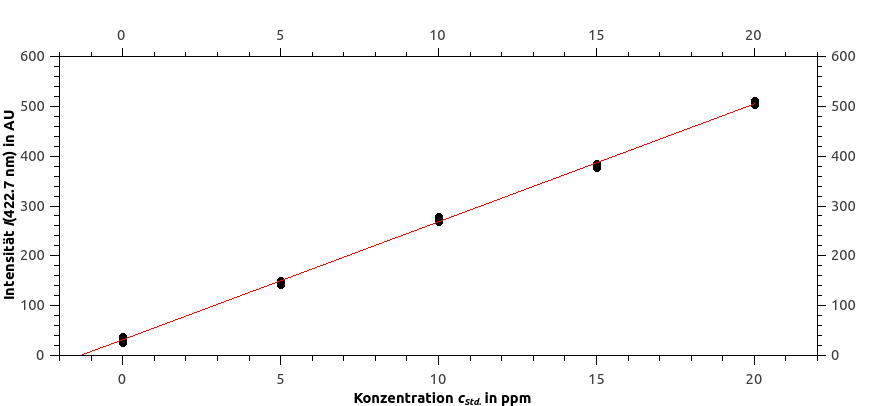
\includegraphics[scale=0.5, center]{images/KalibriergeradeFESCa.png} 
    \caption[Messdaten und Kalibriergerade für die FES von \ch{Ca}, Quelle: Autor]{Messdaten und Kalibriergerade für die FES von \ch{Ca} in der Form $y = a + bx$.}
    \label{fig:KalibriergeradeEisen}
  \end{figure}
  
  \begin{table}[H]
    \centering
    \caption[Ergebnisse der FES-Bestimmung von Calcium, Quelle: Autor]{Ergebnisse der Kalibrier- und Probemessungen bei der FES-Bestimmung von Calcium.}
    
    \label{tab:ErgebnisseFES}
    \begin{tabular}{@{}ll|lp{4.5cm}l@{}}
      \toprule
      Kalibrierstandard Nr. & $c_{Std.}$ in \si{ppm} & $I\left(\SI[mode=text]{422.7}{\nano\meter}\right)$ in AU \\ \midrule
        1 & 0 & 27 \\
        1 & 0 & 34 \\
        1 & 0 & 38 \\
        2 & 5 & 151 \\
        2 & 5 & 145 \\
        2 & 5 & 142 \\
        3 & 10 & 268 \\
        3 & 10 & 273 \\
        3 & 10 & 279 \\
        4 & 15 & 377 \\
        4 & 15 & 384 \\
        4 & 15 & 386 \\
        5 & 20 & 503 \\
        5 & 20 & 505 \\
        5 & 20 & 511 \\ 
          &  &  \\
      \toprule
      Probemessung Nr. & $I\left(\SI[mode=text]{422.7}{\nano\meter}\right)$ in AU & $c_{Probe}$ in \si{ppm} \\ \midrule
        1 & 256 & 9.48 \\
        2 & 262 & 9.74 \\
        3 & 272 & 10.2 \\ 
        4 & 291 & 11.0 \\
        5 & 303 & 11.5 \\ 
        6 & 298 & 11.3 \\ \midrule          
        $\overline{y_i}$ & 280 & 10.5 \\ \bottomrule
    \end{tabular}
  \end{table}
  
  
